\documentclass{beamer}
\mode<presentation>
\usecolortheme{crane}
\setbeamercovered{again covered={\opaqueness<1->{15}}}

\hfuzz=20pt

\input{beamer}
\usepackage{anyfontsize}
\usepackage{fontawesome}
\usepackage{tikz}
\usepackage{filecontents}
\usetikzlibrary{
	positioning
	,plotmarks
	,shapes.callouts	
	,intersections	
}

\tikzset{
	on/.code args={<#1>#2}{
  		\only<#1>{\pgfkeysalso{#2}}
	},
	alt/.code args={<#1>#2#3}{
  		\alt<#1>{\pgfkeysalso{#2}}{\pgfkeysalso{#3}}
	},
}

\tikzset{
	note/.style={rectangle callout, fill=#1}
}

\tikzset{
	label/.style={
		rectangle,	
		draw=none,
		fill=white,
		font=\tiny,
		inner sep=0,
		minimum height=0,
		minimum width=0,
	},
	edge label/.style={
		label,
		midway,
		sloped,
	},
	label below/.style={edge label, below=1mm},
	label above/.style={edge label, above=1mm},
}

\tikzset{default node/.style={
	draw, 
	circle,
	inner sep=0mm,
	minimum size=5mm,
	very thick,
	font=\small,
	black!70,
}}

\tikzset{
	hide/.style={
		opacity=0
	},
	show/.style={
		opacity=1
	},
	hide nodes/.style={
		every node/.append style={hide}
	},
	hide nodes text/.style={
		every node/.append style={text=white}
	},
	show nodes/.style={
		every node/.append style={show}
	},
	show nodes text/.style={
		every node/.append style={text=black}
	},
}

\tikzset{
	>=latex,
	->,
	every node/.style={default node},
}

\tikzset{
	blur/.style={
		black!15
	}
}
\newtheorem{observation}{Observation}

\DeclareMathOperator*{\argmin}{arg\,min}
\DeclareMathOperator*{\argmax}{arg\,max}

\def\R{\mathbb{R}}
\def\N{\mathbb{N}}

\def\1star{{\color{orange} \faStar}}
\def\2star{{\color{orange} \faStar\faStar}}
\def\3star{{\color{orange} \faStar\faStar\faStar}}



\title{Title}
\author[shortname]{
    \textbf{Gilad Kutiel} \inst{1} \and Kutiel Gilad \inst{2}
}
\institute[shortinst]{
    \inst{1} Technion
    \and %
    \inst{2} Technion
}
\date{Conference 2017}

\begin{document}

\input{frame-title}
\begin{frame}{Maximum Carpool Matching (MCM)}
\begin{center}
\begin{tikzpicture}[
every node/.append style={draw=none, font=\large}
, x=1.3cm
, y=1.2cm
, thick
]

% PEOPLE
\begin{scope}[on=<4->{every node/.append style={green}}]
\node(p1) at(0,0) {\faFemale};
\node(p2) at(1,2) {\faFemale};
\node(p3) at(2,0) {\faFemale};
\node(p5) at(4.5,-.5) {\faMale};
\end{scope} 

\begin{scope}[on=<4->{every node/.append style={red}}]
\node(p4) at(3,-2) {\faMale};
\node(p6) at(5,1) {\faMale};
\end{scope}

% VEHICLE
\onslide<2-4>{
\node[below=0 of p4] {\faTruck};
\node[above=0 of p6] {\faCar};
}

\onslide<2-3>{
\node[left=0 of p1] {\faCar};
\node[above=0 of p2] {\faMotorcycle};
\node[below=0 of p3] {\faCab};
\node[below right=0 of p5] {\faMotorcycle};
}

\onslide<3->{
\draw (p1) to[bend right] node[label below]{\2star} (p4);
\draw (p2) to[bend left] node[label above]{\1star} (p6);
\draw (p3) to[bend left] node[label above]{\3star} (p6);
\draw (p5) to[bend right] node[label below]{\2star} (p6);
}

\onslide<3>{
\draw (p1) to[bend left] node[label above]{\1star} (p2);
\draw (p2) to[bend right] node[label below]{\3star} (p3);
\draw (p3) to[bend left] node[label below]{\1star} (p1);
\draw (p3) to[bend right] node[label above]{\1star} (p2);
\draw (p3) to[bend left] node[label above]{\2star} (p4);
\draw (p4) to[bend right] node[label below]{\1star} (p5);
\draw (p6) to[bend left] node[label below]{\2star} (p3);
}



\end{tikzpicture}
\end{center}
\end{frame}
\begin{frame}{Maximum Carpool Matching (MCM) cont.}
\begin{center}
\Huge
Max \3star

s.t. 

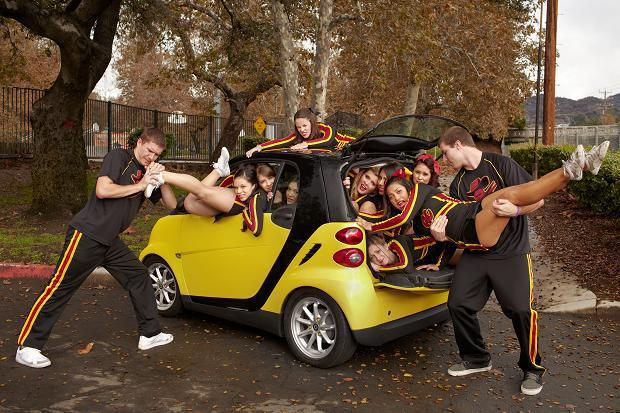
\includegraphics[scale=.3]{capacity}

\onslide<2>{
{\color{green} \faFemale}
{\color{red} \faFemale}
}
\end{center}
\end{frame}
\begin{frame}{Maximum Spanning Star Forest (MSSF)}
\begin{center}
\begin{tikzpicture}[-, thick, x=1.2cm]

\begin{scope}[on=<2>{every node/.append style={green}}]
\node(1) at(0,0){};
\node(3) at(1,2){};
\node(4) at(3,-1){};

\node(6) at(4,2){};
\node(9) at(5,-2){};
\node(10) at(6,2){};
\node(11) at(7,-1){};
\end{scope}

\begin{scope}[on=<2>{every node/.append style={red}}]
\node(2) at(2,1){};
\node(8) at(5,1){};

\node(5) at(1,-3){};
\node(7) at(2,4){};
\end{scope}


\foreach \x/\y in {%
2/1, 2/3, 2/4%
,8/6, 8/9, 8/10, 8/11%
}{
	\draw (\x) -- (\y);
}

\foreach \x/\y in {%
 1/3, 1/4, 1/5%
,3/7, 3/6%
,4/6, 4/9, 4/5%
,5/9%
,6/7, 6/10%
}{
	\draw[on=<2>{blur}] (\x) -- (\y);
}
\end{tikzpicture}
\end{center}
\end{frame}
\begin{frame}{Maximum Spanning Star Forest (MSSF) cont.}
\begin{center}
\Huge
Max \tikz{\node[green, very thick]{};}

s.t.
\tikz{
\node[green, very thick]{};
\node[red, very thick] at(1,0){};
}

\end{center}
\end{frame}
\begin{frame}[<+>]{Hardness}
\begin{itemize}
  \item The problems are APX-hard
  \item $|\text{Dominating Set}| + |\text{SSF}| = |V|$
\end{itemize}
\onslide<+>
\begin{center}
\begin{tikzpicture}[-, thick, x=1cm, y=.7cm]

\begin{scope}[every node/.append style={green}]
\node(1) at(0,0){};
\node(3) at(1,2){};
\node(4) at(3,-1){};

\node(6) at(4,2){};
\node(9) at(5,-2){};
\node(10) at(6,2){};
\node(11) at(7,-1){};
\end{scope}

\begin{scope}[every node/.append style={red}]
\node(2) at(2,1){};
\node(8) at(5,1){};

\node(5) at(1,-3){};
\node(7) at(2,4){};
\end{scope}


\foreach \x/\y in {%
2/1, 2/3, 2/4%
,8/6, 8/9, 8/10, 8/11%
}{
	\draw (\x) -- (\y);
}

\foreach \x/\y in {%
 1/3, 1/4, 1/5%
,3/7, 3/6%
,4/6, 4/9, 4/5%
,5/9%
,6/7, 6/10%
}{
	\draw[blur] (\x) -- (\y);
}
\end{tikzpicture}
\end{center}
\end{frame}
\begin{frame}{Previous Work (MSSF)}
\centering
\begin{tikzpicture}[y=50mm, x=15mm, every node/.style={draw=none}, -]

\draw (6,-5pt) -- (6,1.1) node[anchor=south]{Approximation Ratio};
\draw (5,0) -- (11,0) node[anchor=west]{Year};

\foreach \x in {6,...,10}{
	\draw (\x, 1pt) -- (\x, -3pt) node[anchor=north]{\tiny \x};
}

\foreach \y in {0.25,.5,...,1}{
	\draw (6, \y) -- +(1pt, 0) -- +(-3pt, 0) node[anchor=east]{\tiny \y};
}

\begin{filecontents}{data-upper.txt}
7   0.996153846
8   0.95
8.8 0.91
\end{filecontents}

\begin{filecontents}{data-unweight.txt}
7   0.6
8   0.71
9   0.804
\end{filecontents}

\begin{filecontents}{data-weight-vertex.txt}
8   0.64
9   0.64
\end{filecontents}

\begin{filecontents}{data-weight-edge.txt}
7   0.5
8   0.5
9   0.5
\end{filecontents}

\begin{scope}[every node/.style={note=orange!50}, hide nodes]
\def\pointer{callout absolute pointer}
\node[on=<2>{show}, \pointer={(7,.5)}] at(7, .25)
{\small Nguyen, C. Thach, et al. SODA 2007};

\node[on=<3>{show}, \pointer={(8, .71)}] at(8, 1.3)
{\small Chen, Ning, et al. APPROX 2007};

\node[on=<4>{show}, \pointer={(8.8, .91)}] at(8.8, 1.3)
{\small Deeparnab Chakrabarty et al. FOCS 2008};

\node[on=<5>{show}, \pointer={(9, .804)}] at(9.5, .2)
{\small Athanassopoulos, Stavros, et al. MFCS 2009};
\end{scope}

\tikzset{upper/.style={mark=*, mark options={fill=red}}}
\tikzset{unweight/.style={mark=triangle*, mark options={fill=blue}}}
\tikzset{weight-vertex/.style={mark=square*, mark options={fill=cyan}}}
\tikzset{weight-edge/.style={mark=diamond*, mark options={fill=green}}}

\draw plot[upper] file {data-upper.txt};
\draw plot[unweight] file {data-unweight.txt};
\draw plot[weight-vertex] file {data-weight-vertex.txt}; 
\draw plot[weight-edge] file {data-weight-edge.txt};


\draw 
plot[upper] (10,1) -- +(-5pt,0) -- +(5pt,0) 
node[right]{\tiny Hardness};

\draw[yshift=-\baselineskip] 
plot[unweight] (10,1) -- +(-5pt,0) -- +(5pt,0) 
node[right]{\tiny Unweighted};

\draw[yshift=-2\baselineskip] 
plot[weight-vertex] (10,1) -- +(-5pt,0) -- +(5pt,0) 
node[right]{\tiny Vertex Weighted};

\draw[yshift=-3\baselineskip] 
plot[weight-edge] (10,1) -- +(-5pt,0) -- +(5pt,0) 
node[right]{\tiny Edge Weighted};

\end{tikzpicture}
\end{frame}
\begin{frame}{Previous Work (MCM)}
\begin{itemize}[<+>]
	\item The algorithms for MSSF do not generalize to MCM  
	\item<+-+(1)> Heuristics + experiments
  		\begin{itemize}[<+>]
  			\item Solution's quality \alert{matters}
		\end{itemize}
	\item<+-+(2)> Kutiel
	\begin{itemize}
		\item $1/3$-approximation 
		\item $1/2$-approximation (unweighted) 
	\end{itemize}
\end{itemize}
\end{frame}
\begin{frame}[<+>]{Our Results}
\begin{itemize}
  	\item APX-hard for bounded degree graphs 
	\item<+-+(1)> MCM as submodular maximization (David Adjashvili) 
		\begin{itemize}
		  \item $1/2$-approximation 
		\end{itemize}
	\item $(1/2 - \varepsilon)$-approximation (local search)
	\item<+-+(1)> Group Carpool (not submodular)
		\begin{itemize}
			\item $(1/2 - \varepsilon)$-approximation (local search)
		\end{itemize}
	\item $1/2 + 1/2k - \varepsilon$-approximation (unweighted, $k$ = max degree)
\end{itemize}
\end{frame}
\begin{frame}{Fixed Matching}
\begin{center}
\begin{tikzpicture}[every node/.append style={draw=none, font=\large},thick]

\onslide<+->
% NODES 
\foreach[count=\i] \x/\y/\c in {%
0/0/blue%
, 2/1/brown%
, 1/2/blue%
, 3.5/-.5/brown%
, 4/2/blue%
, 5.5/1/brown%
, 7/0/blue%
}{
\node[\c](\i) at(\x,\y) {\faFemale};
}

\onslide<+->
% CARS
\begin{scope}[every node/.style={label}]
\foreach \i/\p/\fa in {%
1/left/\faCar%
,2/below/\faMotorcycle%
,3/above/\faCar%
,4/below/\faCab%
,5/above/\faCar%
,6/above right/\faTruck%
,7/right/\faMotorcycle%
}{
\node[\p=0 of \i]{\small\fa};
} 
\end{scope} 

% ARCS 
\foreach \i/\j/\s in {%
1/2/\3star%
, 1/3/\1star%
, 2/3/\2star%
, 2/4/\1star%
, 2/5/\3star%
, 3/5/\1star%
, 4/1/\1star%
, 4/5/\2star%
, 4/6/\1star%
, 5/6/\2star%
, 7/6/\1star%
, 7/4/\1star%
}{
\draw (\i) -- (\j) node[label above] {\Tiny \s};
}

\onslide<+->
% FLOW
\begin{scope}[yshift=-5.5cm]


% LEFT NODES
\begin{scope}[y=.9cm]
\foreach[count=\i] \id in {1,3,7,5}{
\node[blue](f\id) at(2, \i) {\faFemale};
}
\end{scope}

% RIGHT NODES
\begin{scope}[y=1.25cm, yshift=-.25cm]
\foreach[count=\i] \id in {2,4,6}{
\node[brown](f\id) at(4.5, \i) {\faFemale};
}
\end{scope}

\foreach \i/\j/\s in {%
1/2/\3star%
,5/6/\2star%
,7/6/\1star%
,7/4/\1star%
}{
\draw (f\i) -- (f\j) node[label above] {1/\s};
}


\node(s) at (-.5, 2.25) {s};
\node(t) at (7, 2.25) {t};

% S - LEFT
\draw (s) -- (f5) node[label above]{1/0};

\foreach \i in {1,3,7}{
\draw[dashed, thin, black!50] (s) -- (f\i);
}

% RIGHT - T
\foreach \i/\c in {%
2/\faMotorcycle%
,4/\faCab%
,6/\faTruck%
}{
\draw (f\i) -- (t) node[label above]{\c/0};
}


\end{scope}

\end{tikzpicture}
\end{center}
\end{frame}
\begin{frame}{Submodular}
\begin{itemize}[<+>]
  \item Let $D = \{{\color{brown}\text{\faFemale}, \ldots, \text{\faFemale}}\} \subseteq V$
  \item Let $F(D) = OPT$ (w.r.t D)
\end{itemize}

\onslide<+>
\begin{theorem}
$F$ is submodular
\end{theorem}

\onslide<+>
\begin{corollary}
MCM is $1/2$-approximable
\end{corollary}



\end{frame}
\begin{frame}{Submodular cont.}
\begin{center}
\begin{tikzpicture}[
every node/.append style={
	draw=none, 
	blue, 
	font=\Large
}
, y=1.5cm
, x=1.5cm
, very thick
]

\def\group#1#2#3{
\draw[#3, -]
(#1.west)
to[out=90,in=90] (#2.east)
to[out=-90,in=-90] (#1.west)
;
}

% GROUP 1 
\node(11) at(0,1){\faFemale};
\node(12) at(1,1){\faFemale};
\node(13) at(2,1){\faFemale};

\begin{scope}[every node/.append style={brown}]
\node(14) at(0,0){\faFemale};
\node(15) at(1,0){\faFemale};
\node(16) at(2,0){\faFemale};
\end{scope}

\group{14}{15}{purple}
\group{15}{16}{cyan}

\draw[green] (11) -- (14);
\draw (12) -- (15);
\draw[orange] (13) -- (16);

% GROUP 2 
\begin{scope}[yshift=-4cm]
\node(21) at(0,1){\faFemale};
\node(22) at(1,1){\faFemale};
\node(23) at(2,1){\faFemale};
\node(24) at(0,0){\faFemale};

\begin{scope}[every node/.append style={brown}]
\node(25) at(1,0){\faFemale};
\end{scope}

\node(26) at(2,0){\faFemale};
\end{scope}

\draw[] (21) -- (25);
\draw[orange] (24) -- (25);
\draw[green] (26) -- (25);


% GROUP 3 
\begin{scope}[xshift=7cm]
\node(41) at(0,1){\faFemale};
\node(42) at(1,1){\faFemale};
\node(43) at(2,1){\faFemale};

\begin{scope}[every node/.append style={brown}]
\node(44) at(0,0){\faFemale};
\node(45) at(1,0){\faFemale};
\end{scope}

\node(46) at(2,0){\faFemale};
\end{scope}

\group{44}{45}{purple}

\draw[green] (41) -- (44);
\draw (42) -- (45);
\draw[green] (46) -- (45);


% GROUP 4 
\begin{scope}[xshift=7cm, yshift=-4cm]
\node(31) at(0,1){\faFemale};
\node(32) at(1,1){\faFemale};
\node(33) at(2,1){\faFemale};

\node(34) at(0,0){\faFemale};

\begin{scope}[every node/.append style={brown}]
\node(35) at(1,0){\faFemale};
\node(36) at(2,0){\faFemale};
\end{scope}

\end{scope}

\group{35}{36}{cyan}

\draw (31) -- (35);
\draw[orange] (34) -- (35);
\draw[orange] (33) -- (36);


\end{tikzpicture}
\end{center}
\end{frame}
\begin{frame}{Local Search - Unweighted, $|\text{\faTruck}| = O(1)$}
\begin{itemize}[<+>]
  \item For a fixed $K$
  \item Start with any solution
  \item<+-+(2)> while possible
  	\begin{itemize}
  	  \item Remove $k \leq K$ arcs
  	  \item Add at least $k+1$
	\end{itemize}
\end{itemize}
\end{frame}
\begin{frame}{Local Search - Analysis (Star Graph)}
\begin{columns}
\begin{column}{1.2\textwidth}
\begin{center}
\begin{tikzpicture}[thick, x=.9cm, every node/.append style={draw=none}]

\onslide<+->
% NODES
\foreach[count=\i] \x/\y in {%
0/0, 2/1, 1/2, 2/-2, 3/-1, 1.5/-.5,4/1.5,5/0,4/-3,5/-1.5%
}{
\node(\i) at(\x,\y) {\large\faFemale};
}

\onslide<+->
% OPTIMAL
\foreach \i/\j in{%
1/2,3/2%
,6/4,5/4%
,7/8,10/8%
}{
\draw[red] (\i) -- (\j);
}

\onslide<+->
% ALG
\foreach \i/\j in{%
6/1,3/1%
,2/5%
,9/10%
}{
\draw[green] (\i) -- (\j);
}

\onslide<+->
% OUTLINE
\draw[blue, dashed, -] 
(4.south)
to [out=180,in=225] (6.north west)
to [out=45,in=135] (5.north east)
to [out=-45,in=0] (4.south)
;

\draw[blue, dashed, -] 
(1.south)
to [out=180,in=180] (3.north)
to [out=0,in=90] (2.east)
to [out=-90,in=0] (1.south)
;

\draw[blue, dashed, -] 
(10.south)
to [out=180,in=180] (7.north)
to [out=0,in=90] (8.east)
to [out=-90,in=0] (10.south)
;

\draw[blue, dashed, -] 
(9.south)
to [out=180,in=180] (9.north)
to [out=0,in=0] (9.south)
;

\onslide<+->
% STARS
\begin{scope}[xshift=6cm]
\foreach[count=\i] \x/\y in {%
2/1, 2/-2,5/0,4/-3%
}{
\node[red](s\i) at(\x,\y) {\large\faStar};
}
\end{scope}

% EDGES
\foreach \i/\j in{%
1/2,4/3%
}{
\draw[green, -] (s\i) -- (s\j);
}

\end{tikzpicture}
\end{center}
\end{column}
\end{columns}
\end{frame}
\begin{frame}{Local Search - Star Graph}
\begin{center}
\begin{tikzpicture}[
every node/.append style={draw=none, font=\Large}
, y=0.8cm
, -
, very thick
]
\foreach[count=\i] \x/\y in {%
0/0, 2/1, 1/2, 4/-1, 5/2, 7/0, 3/4, 4/5, 7/5, 8/3%
}{
\node[red](\i) at(\x,\y) {\faStar \i};
}

\foreach \i/\j in {%
1/2, 2/3, 3/7, 7/8, 2/4, 4/5, 5/6, 4/6, 9/10, 5/7%
}{
\draw[green] (\i) -- (\j) coordinate[midway](\i\j);
}

\draw[blue, dashed, thick] 
(4.west) 
to[out=90,in=180] (5.north)
to[out=0, in=90] (6.east)
to[out=270, in=270] (4.west)
;

\draw[blue, dashed, thick] 
(1.west) 
to[out=90,in=180] (3.north)
to[out=0, in=90] (2.east)
to[out=270, in=270] (1.west)
;

\draw[blue, dashed, thick] 
(7.south west) 
to[out=180,in=180] (8.north east)
to[out=0, in=0] (7.south west)
;

\draw[blue, dashed, thick] 
(10.south) 
to[out=180,in=180] (9.north)
to[out=0, in=0] (10.south)
;

\begin{scope}[every node/.style={note=orange!50}]
\def\pointer{callout absolute pointer}

\node[\pointer={(1.south)}] at(0, -2)
{\small An optimal star};

\node[\pointer={(37)}] at(0, 4)
{\small Alg arc};

\end{scope}

\end{tikzpicture}
\end{center}
\end{frame}
\begin{frame}{Local Search - Rough Analysis}
\begin{columns}
\begin{column}{.63\textwidth}

\begin{itemize}[<+->]
\item Let $r := \frac{\#\text{\color{red}\faStar}}{\#\text{Good edges}}$ 
	\item Each {\color{red}\faStar} intersects with (on averege):
	\begin{itemize}
% 	  \item contribute $\color{red} \leq |\text{\faTruck}|$ to OPT
	  \item $r$ good edges
	  \item $\geq |\text{\color{red}\faStar}| - r$ bad edges
	\end{itemize}
	\item Roughly, for large $K$, $r \geq 1$
\end{itemize}
\end{column}
\begin{column}{.49\textwidth}
\begin{tikzpicture}[very thick, every node/.append style={draw=none, font=\Large}]
\foreach[count=\i] \x/\y in {%
0/0, 1/2, 2/1%
}{
\node[red](\i) at(\x,\y){\faStar\i};
}

\foreach \i/\j in {%
1/2,2/3%
}{
\draw[green,-] (\i) -- (\j);
}

\draw[blue, dashed, -]
(1.south)
to[out=180, in=180] (2.north)
to[out=0, in=90] (3.east)
to[out=-90, in=0] (1.south)
;

\foreach[count=\i] \l in {%
2cm, 1cm, 0% 
}{
\node(bl\i) at(1)[below left=1.5cm and \l] {};
\draw[green,-] (1) -- (bl\i);
}
\end{tikzpicture}
\end{column}
\end{columns}

\onslide<+->
\vfill
$$
\frac{\color{green} r + 1/2 (|\text{\faStar}| - r)}
{\color{red} |\text{\faStar}|} 
\onslide<+->
\geq
\onslide<+->
\frac{\color{green} 1 + 1/2 (|\text{\faStar}| - 1)}
{\color{red} |\text{\faStar}|} 
\onslide<+->
=
\bm{\frac{1}{2} + \frac{1}{2 |\text{\faTruck}|}}
$$
\end{frame}



\begin{frame}{Summary}
\begin{itemize}[<+->]
  \item APX-hardness for bounded degree graphs
  \item \alert{MCM is submodular}
  	\begin{itemize}
  	\item 1/2-approximation
	\end{itemize}
  \item Group Carpool
  	\begin{itemize}
  	  \item Not Submodular
  	  \item $(1/2-\varepsilon)$-approximation
	\end{itemize}
  \item \alert{better approximation if unweighted}
  \item Is 1/2 the best we can hope for ?
\end{itemize}
\end{frame}
\input{frame-thank-you}

\end{document}